% Options for packages loaded elsewhere
\PassOptionsToPackage{unicode}{hyperref}
\PassOptionsToPackage{hyphens}{url}
%
\documentclass[
]{article}
\usepackage{amsmath,amssymb}
\usepackage{lmodern}
\usepackage{iftex}
\ifPDFTeX
  \usepackage[T1]{fontenc}
  \usepackage[utf8]{inputenc}
  \usepackage{textcomp} % provide euro and other symbols
\else % if luatex or xetex
  \usepackage{unicode-math}
  \defaultfontfeatures{Scale=MatchLowercase}
  \defaultfontfeatures[\rmfamily]{Ligatures=TeX,Scale=1}
\fi
% Use upquote if available, for straight quotes in verbatim environments
\IfFileExists{upquote.sty}{\usepackage{upquote}}{}
\IfFileExists{microtype.sty}{% use microtype if available
  \usepackage[]{microtype}
  \UseMicrotypeSet[protrusion]{basicmath} % disable protrusion for tt fonts
}{}
\makeatletter
\@ifundefined{KOMAClassName}{% if non-KOMA class
  \IfFileExists{parskip.sty}{%
    \usepackage{parskip}
  }{% else
    \setlength{\parindent}{0pt}
    \setlength{\parskip}{6pt plus 2pt minus 1pt}}
}{% if KOMA class
  \KOMAoptions{parskip=half}}
\makeatother
\usepackage{xcolor}
\usepackage[margin=1in]{geometry}
\usepackage{color}
\usepackage{fancyvrb}
\newcommand{\VerbBar}{|}
\newcommand{\VERB}{\Verb[commandchars=\\\{\}]}
\DefineVerbatimEnvironment{Highlighting}{Verbatim}{commandchars=\\\{\}}
% Add ',fontsize=\small' for more characters per line
\usepackage{framed}
\definecolor{shadecolor}{RGB}{248,248,248}
\newenvironment{Shaded}{\begin{snugshade}}{\end{snugshade}}
\newcommand{\AlertTok}[1]{\textcolor[rgb]{0.94,0.16,0.16}{#1}}
\newcommand{\AnnotationTok}[1]{\textcolor[rgb]{0.56,0.35,0.01}{\textbf{\textit{#1}}}}
\newcommand{\AttributeTok}[1]{\textcolor[rgb]{0.77,0.63,0.00}{#1}}
\newcommand{\BaseNTok}[1]{\textcolor[rgb]{0.00,0.00,0.81}{#1}}
\newcommand{\BuiltInTok}[1]{#1}
\newcommand{\CharTok}[1]{\textcolor[rgb]{0.31,0.60,0.02}{#1}}
\newcommand{\CommentTok}[1]{\textcolor[rgb]{0.56,0.35,0.01}{\textit{#1}}}
\newcommand{\CommentVarTok}[1]{\textcolor[rgb]{0.56,0.35,0.01}{\textbf{\textit{#1}}}}
\newcommand{\ConstantTok}[1]{\textcolor[rgb]{0.00,0.00,0.00}{#1}}
\newcommand{\ControlFlowTok}[1]{\textcolor[rgb]{0.13,0.29,0.53}{\textbf{#1}}}
\newcommand{\DataTypeTok}[1]{\textcolor[rgb]{0.13,0.29,0.53}{#1}}
\newcommand{\DecValTok}[1]{\textcolor[rgb]{0.00,0.00,0.81}{#1}}
\newcommand{\DocumentationTok}[1]{\textcolor[rgb]{0.56,0.35,0.01}{\textbf{\textit{#1}}}}
\newcommand{\ErrorTok}[1]{\textcolor[rgb]{0.64,0.00,0.00}{\textbf{#1}}}
\newcommand{\ExtensionTok}[1]{#1}
\newcommand{\FloatTok}[1]{\textcolor[rgb]{0.00,0.00,0.81}{#1}}
\newcommand{\FunctionTok}[1]{\textcolor[rgb]{0.00,0.00,0.00}{#1}}
\newcommand{\ImportTok}[1]{#1}
\newcommand{\InformationTok}[1]{\textcolor[rgb]{0.56,0.35,0.01}{\textbf{\textit{#1}}}}
\newcommand{\KeywordTok}[1]{\textcolor[rgb]{0.13,0.29,0.53}{\textbf{#1}}}
\newcommand{\NormalTok}[1]{#1}
\newcommand{\OperatorTok}[1]{\textcolor[rgb]{0.81,0.36,0.00}{\textbf{#1}}}
\newcommand{\OtherTok}[1]{\textcolor[rgb]{0.56,0.35,0.01}{#1}}
\newcommand{\PreprocessorTok}[1]{\textcolor[rgb]{0.56,0.35,0.01}{\textit{#1}}}
\newcommand{\RegionMarkerTok}[1]{#1}
\newcommand{\SpecialCharTok}[1]{\textcolor[rgb]{0.00,0.00,0.00}{#1}}
\newcommand{\SpecialStringTok}[1]{\textcolor[rgb]{0.31,0.60,0.02}{#1}}
\newcommand{\StringTok}[1]{\textcolor[rgb]{0.31,0.60,0.02}{#1}}
\newcommand{\VariableTok}[1]{\textcolor[rgb]{0.00,0.00,0.00}{#1}}
\newcommand{\VerbatimStringTok}[1]{\textcolor[rgb]{0.31,0.60,0.02}{#1}}
\newcommand{\WarningTok}[1]{\textcolor[rgb]{0.56,0.35,0.01}{\textbf{\textit{#1}}}}
\usepackage{longtable,booktabs,array}
\usepackage{calc} % for calculating minipage widths
% Correct order of tables after \paragraph or \subparagraph
\usepackage{etoolbox}
\makeatletter
\patchcmd\longtable{\par}{\if@noskipsec\mbox{}\fi\par}{}{}
\makeatother
% Allow footnotes in longtable head/foot
\IfFileExists{footnotehyper.sty}{\usepackage{footnotehyper}}{\usepackage{footnote}}
\makesavenoteenv{longtable}
\usepackage{graphicx}
\makeatletter
\def\maxwidth{\ifdim\Gin@nat@width>\linewidth\linewidth\else\Gin@nat@width\fi}
\def\maxheight{\ifdim\Gin@nat@height>\textheight\textheight\else\Gin@nat@height\fi}
\makeatother
% Scale images if necessary, so that they will not overflow the page
% margins by default, and it is still possible to overwrite the defaults
% using explicit options in \includegraphics[width, height, ...]{}
\setkeys{Gin}{width=\maxwidth,height=\maxheight,keepaspectratio}
% Set default figure placement to htbp
\makeatletter
\def\fps@figure{htbp}
\makeatother
\setlength{\emergencystretch}{3em} % prevent overfull lines
\providecommand{\tightlist}{%
  \setlength{\itemsep}{0pt}\setlength{\parskip}{0pt}}
\setcounter{secnumdepth}{-\maxdimen} % remove section numbering
\usepackage{booktabs}
\usepackage{longtable}
\usepackage{array}
\usepackage{multirow}
\usepackage{wrapfig}
\usepackage{float}
\usepackage{colortbl}
\usepackage{pdflscape}
\usepackage{tabu}
\usepackage{threeparttable}
\usepackage{threeparttablex}
\usepackage[normalem]{ulem}
\usepackage{makecell}
\usepackage{xcolor}
\ifLuaTeX
  \usepackage{selnolig}  % disable illegal ligatures
\fi
\IfFileExists{bookmark.sty}{\usepackage{bookmark}}{\usepackage{hyperref}}
\IfFileExists{xurl.sty}{\usepackage{xurl}}{} % add URL line breaks if available
\urlstyle{same} % disable monospaced font for URLs
\hypersetup{
  pdftitle={Simulation Experiment Results},
  pdfauthor={Victor Tsang (z5209633)},
  hidelinks,
  pdfcreator={LaTeX via pandoc}}

\title{Simulation Experiment Results}
\author{Victor Tsang (z5209633)}
\date{2022-11-14}

\begin{document}
\maketitle

\hypertarget{load-in-the-results}{%
\subsubsection{Load in the results}\label{load-in-the-results}}

\begin{Shaded}
\begin{Highlighting}[]
\FunctionTok{library}\NormalTok{(knitr)}
\FunctionTok{library}\NormalTok{(tidyverse)}

\FunctionTok{library}\NormalTok{(gridExtra)}
\FunctionTok{library}\NormalTok{(latex2exp)}

\FunctionTok{load}\NormalTok{(}\StringTok{"../data/synthetic{-}data.RData"}\NormalTok{)}
\FunctionTok{attach}\NormalTok{(synthetic.data.config)}
\end{Highlighting}
\end{Shaded}

\hypertarget{cleaning-up-and-renaming-things}{%
\subsubsection{Cleaning up and renaming
things}\label{cleaning-up-and-renaming-things}}

\begin{Shaded}
\begin{Highlighting}[]
\NormalTok{estimates }\OtherTok{=} \FunctionTok{readRDS}\NormalTok{(}\StringTok{"../data/sim\_exp{-}estimate\_extinction\_results.RDS"}\NormalTok{)}
\NormalTok{estimates }\OtherTok{=}\NormalTok{ estimates }\SpecialCharTok{\%\textgreater{}\%} \FunctionTok{filter}\NormalTok{(}\SpecialCharTok{!}\NormalTok{(method }\SpecialCharTok{\%in\%} \FunctionTok{c}\NormalTok{(}\StringTok{"SI{-}RM"}\NormalTok{, }\StringTok{"GB{-}RM"}\NormalTok{)))}
\NormalTok{estimates }\OtherTok{=}\NormalTok{ estimates }\SpecialCharTok{\%\textgreater{}\%} \FunctionTok{mutate}\NormalTok{(}\FunctionTok{across}\NormalTok{(method, str\_replace, }\StringTok{\textquotesingle{}SI{-}RM{-}corrected\textquotesingle{}}\NormalTok{, }\StringTok{\textquotesingle{}SI{-}RM\textquotesingle{}}\NormalTok{),}
                                 \AttributeTok{method\_cat =} \FunctionTok{ifelse}\NormalTok{(method }\SpecialCharTok{\%in\%} \FunctionTok{c}\NormalTok{(}\StringTok{"SI{-}RM"}\NormalTok{, }\StringTok{"MINMI"}\NormalTok{),}
                                                     \StringTok{"Proposed"}\NormalTok{,}
                                                     \StringTok{"Existing"}\NormalTok{),}
                                 \AttributeTok{method =} \FunctionTok{ifelse}\NormalTok{(method }\SpecialCharTok{==} \StringTok{"GRIWM"}\NormalTok{,}
                                                 \StringTok{"GRIWM (q=0.05)"}\NormalTok{,}
                                                 \FunctionTok{ifelse}\NormalTok{(method }\SpecialCharTok{==} \StringTok{"GRIWM{-}corrected"}\NormalTok{,}
                                                        \StringTok{"GRIWM{-}BA (q=0.5)"}\NormalTok{,}
                                                        \FunctionTok{ifelse}\NormalTok{(method }\SpecialCharTok{==} \StringTok{"STRAUSS"}\NormalTok{,}
                                                          \StringTok{"Strauss"}\NormalTok{,}
\NormalTok{                                                          method}
\NormalTok{                                                        ))))}
\NormalTok{estimates }\OtherTok{=}\NormalTok{ estimates }\SpecialCharTok{\%\textgreater{}\%} \FunctionTok{filter}\NormalTok{(error\_factor }\SpecialCharTok{!=} \DecValTok{4}\NormalTok{)}
\FunctionTok{head}\NormalTok{(estimates)}
\end{Highlighting}
\end{Shaded}

\begin{verbatim}
##   id error_factor method     lower     point    upper point_runtime
## 1  1          0.0    MLE        NA 12660.896       NA  1.907349e-05
## 2  1          0.0 BA-MLE        NA 12293.940       NA  1.682997e-03
## 3  1          0.0 SI-UGM 11262.804 12422.265 12681.61  3.777524e+00
## 4  2          0.5    MLE        NA  9871.056       NA  1.279831e-03
## 5  2          0.5 BA-MLE        NA  9364.609       NA  4.145861e-03
## 6  2          0.5 SI-UGM  7789.998  9518.421 10035.51  2.695084e+00
##   conf_int_runtime B.point B.lower B.upper method_cat
## 1               NA      NA      NA      NA   Existing
## 2               NA      NA      NA      NA   Existing
## 3         3.777524      NA      NA      NA   Existing
## 4               NA      NA      NA      NA   Existing
## 5               NA      NA      NA      NA   Existing
## 6         2.695084      NA      NA      NA   Existing
\end{verbatim}

\begin{Shaded}
\begin{Highlighting}[]
\CommentTok{\# Point estimates}
\NormalTok{performance.point\_estimates }\OtherTok{=}\NormalTok{ estimates }\SpecialCharTok{\%\textgreater{}\%}
  \FunctionTok{filter}\NormalTok{(}\SpecialCharTok{!}\FunctionTok{is.na}\NormalTok{(point)) }\SpecialCharTok{\%\textgreater{}\%}
  \FunctionTok{group\_by}\NormalTok{(error\_factor, method, method\_cat) }\SpecialCharTok{\%\textgreater{}\%}
  \FunctionTok{summarise}\NormalTok{(}\AttributeTok{MSE\_000 =} \FunctionTok{mean}\NormalTok{((point }\SpecialCharTok{{-}}\NormalTok{ theta.true)}\SpecialCharTok{\^{}}\DecValTok{2}\NormalTok{)}\SpecialCharTok{/}\DecValTok{1000}\NormalTok{,}
            \AttributeTok{bias =} \FunctionTok{mean}\NormalTok{(point)}\SpecialCharTok{{-}}\NormalTok{theta.true,}
            \AttributeTok{variance\_000 =} \FunctionTok{var}\NormalTok{(point)}\SpecialCharTok{/}\DecValTok{1000}\NormalTok{,}
            \AttributeTok{avg\_runtime =} \FunctionTok{round}\NormalTok{(}\FunctionTok{mean}\NormalTok{(point\_runtime), }\DecValTok{5}\NormalTok{))}
\end{Highlighting}
\end{Shaded}

\begin{verbatim}
## `summarise()` has grouped output by 'error_factor', 'method'. You can override
## using the `.groups` argument.
\end{verbatim}

\begin{Shaded}
\begin{Highlighting}[]
\FunctionTok{kable}\NormalTok{(performance.point\_estimates)}
\end{Highlighting}
\end{Shaded}

\begin{longtable}[]{@{}
  >{\raggedleft\arraybackslash}p{(\columnwidth - 12\tabcolsep) * \real{0.1444}}
  >{\raggedright\arraybackslash}p{(\columnwidth - 12\tabcolsep) * \real{0.1889}}
  >{\raggedright\arraybackslash}p{(\columnwidth - 12\tabcolsep) * \real{0.1222}}
  >{\raggedleft\arraybackslash}p{(\columnwidth - 12\tabcolsep) * \real{0.1111}}
  >{\raggedleft\arraybackslash}p{(\columnwidth - 12\tabcolsep) * \real{0.1556}}
  >{\raggedleft\arraybackslash}p{(\columnwidth - 12\tabcolsep) * \real{0.1444}}
  >{\raggedleft\arraybackslash}p{(\columnwidth - 12\tabcolsep) * \real{0.1333}}@{}}
\toprule()
\begin{minipage}[b]{\linewidth}\raggedleft
error\_factor
\end{minipage} & \begin{minipage}[b]{\linewidth}\raggedright
method
\end{minipage} & \begin{minipage}[b]{\linewidth}\raggedright
method\_cat
\end{minipage} & \begin{minipage}[b]{\linewidth}\raggedleft
MSE\_000
\end{minipage} & \begin{minipage}[b]{\linewidth}\raggedleft
bias
\end{minipage} & \begin{minipage}[b]{\linewidth}\raggedleft
variance\_000
\end{minipage} & \begin{minipage}[b]{\linewidth}\raggedleft
avg\_runtime
\end{minipage} \\
\midrule()
\endhead
0.0 & BA-MLE & Existing & 234.5607 & -0.9379571 & 234.7946 & 0.00002 \\
0.0 & GRIWM-BA (q=0.5) & Existing & 246.1900 & 133.7070000 & 228.5410 &
13.89881 \\
0.0 & GRIWM (q=0.05) & Existing & 1183.5359 & -949.8850000 & 281.5360 &
2.33548 \\
0.0 & MINMI & Proposed & 247.4576 & 139.4092643 & 228.2509 & 0.00001 \\
0.0 & MLE & Existing & 438.6601 & 475.2971837 & 212.9656 & 0.00002 \\
0.0 & SI-RM & Proposed & 438.6601 & 475.2971837 & 212.9656 & 0.05641 \\
0.0 & SI-UGM & Existing & 248.9648 & 150.6138962 & 226.5068 & 4.70657 \\
0.0 & Strauss & Existing & 234.8453 & -0.7152842 & 235.0799 & 0.00002 \\
0.5 & BA-MLE & Existing & 244.0353 & -22.0990141 & 243.7908 & 0.00003 \\
0.5 & GRIWM-BA (q=0.5) & Existing & 244.7798 & 95.1730000 & 235.9578 &
13.88254 \\
0.5 & GRIWM (q=0.05) & Existing & 1275.8894 & -992.6550000 & 290.8162 &
2.35887 \\
0.5 & MINMI & Proposed & 253.0606 & 118.8454210 & 239.1755 & 0.00047 \\
0.5 & MLE & Existing & 428.0602 & 455.1437961 & 221.1254 & 0.00002 \\
0.5 & SI-RM & Proposed & 428.0602 & 455.1437961 & 221.1254 & 0.06072 \\
0.5 & SI-UGM & Existing & 250.7756 & 117.2579537 & 237.2634 & 2.33059 \\
0.5 & Strauss & Existing & 245.5802 & -22.8493286 & 245.3034 &
0.00002 \\
1.0 & BA-MLE & Existing & 365.6242 & -45.7554617 & 363.8946 & 0.00002 \\
1.0 & GRIWM-BA (q=0.5) & Existing & 345.2420 & 34.4120000 & 344.4022 &
13.90095 \\
1.0 & GRIWM (q=0.05) & Existing & 1547.7470 & -1060.0020000 & 424.5673 &
18.10725 \\
1.0 & MINMI & Proposed & 373.3208 & 103.7670782 & 362.9161 & 0.00057 \\
1.0 & MLE & Existing & 516.8878 & 432.6138460 & 330.0631 & 0.00002 \\
1.0 & SI-RM & Proposed & 516.8878 & 432.6138460 & 330.0631 & 0.05992 \\
1.0 & SI-UGM & Existing & 371.3002 & 115.2129004 & 358.3845 & 1.93741 \\
1.0 & Strauss & Existing & 366.4727 & -50.5383309 & 364.2829 &
0.00002 \\
2.0 & BA-MLE & Existing & 542.9867 & -233.5215118 & 488.9434 &
0.00002 \\
2.0 & GRIWM-BA (q=0.5) & Existing & 504.9335 & -278.4774775 & 427.8120 &
13.94220 \\
2.0 & GRIWM (q=0.05) & Existing & 2506.9717 & -1407.5250000 & 526.3714 &
2.36410 \\
2.0 & MINMI & Proposed & 491.9000 & 27.3303294 & 491.6447 & 0.00071 \\
2.0 & MLE & Existing & 507.4514 & 253.7890364 & 443.4860 & 0.00002 \\
2.0 & SI-RM & Proposed & 507.4514 & 253.7890364 & 443.4860 & 0.05993 \\
2.0 & SI-UGM & Existing & 501.5358 & 65.3780494 & 497.7593 & 1.68008 \\
2.0 & Strauss & Existing & 553.8156 & -247.9251968 & 492.8416 &
0.00002 \\
\bottomrule()
\end{longtable}

\begin{Shaded}
\begin{Highlighting}[]
\CommentTok{\# Confidence Intervals}
\NormalTok{performance.conf\_int\_estimates }\OtherTok{=}\NormalTok{ estimates }\SpecialCharTok{\%\textgreater{}\%}
  \FunctionTok{filter}\NormalTok{(}\SpecialCharTok{!}\FunctionTok{is.na}\NormalTok{(conf\_int\_runtime)) }\SpecialCharTok{\%\textgreater{}\%}
  \FunctionTok{mutate}\NormalTok{(}\AttributeTok{width =}\NormalTok{ upper }\SpecialCharTok{{-}}\NormalTok{ lower,}
         \AttributeTok{contains\_theta =} \FunctionTok{ifelse}\NormalTok{(theta.true }\SpecialCharTok{\textgreater{}}\NormalTok{ lower }\SpecialCharTok{\&}\NormalTok{ theta.true }\SpecialCharTok{\textless{}}\NormalTok{ upper, }\DecValTok{1}\NormalTok{, }\DecValTok{0}\NormalTok{)) }\SpecialCharTok{\%\textgreater{}\%}
  \FunctionTok{group\_by}\NormalTok{(error\_factor, method, method\_cat) }\SpecialCharTok{\%\textgreater{}\%}
  \FunctionTok{summarise}\NormalTok{(}\AttributeTok{Coverage =} \FunctionTok{round}\NormalTok{(}\FunctionTok{mean}\NormalTok{(contains\_theta) }\SpecialCharTok{*} \DecValTok{100}\NormalTok{, }\DecValTok{1}\NormalTok{),}
            \StringTok{\textasciigrave{}}\AttributeTok{Average Width}\StringTok{\textasciigrave{}} \OtherTok{=} \FunctionTok{round}\NormalTok{(}\FunctionTok{mean}\NormalTok{(width), }\DecValTok{2}\NormalTok{),}
            \StringTok{\textasciigrave{}}\AttributeTok{Average Runtime}\StringTok{\textasciigrave{}} \OtherTok{=} \FunctionTok{round}\NormalTok{(}\FunctionTok{mean}\NormalTok{(conf\_int\_runtime), }\DecValTok{4}\NormalTok{)) }\SpecialCharTok{\%\textgreater{}\%}
  \FunctionTok{ungroup}\NormalTok{() }\SpecialCharTok{\%\textgreater{}\%}
  \FunctionTok{arrange}\NormalTok{(}\FunctionTok{desc}\NormalTok{(Coverage), }\StringTok{\textasciigrave{}}\AttributeTok{Average Width}\StringTok{\textasciigrave{}}\NormalTok{, }\StringTok{\textasciigrave{}}\AttributeTok{Average Runtime}\StringTok{\textasciigrave{}}\NormalTok{)}
\end{Highlighting}
\end{Shaded}

\begin{verbatim}
## `summarise()` has grouped output by 'error_factor', 'method'. You can override
## using the `.groups` argument.
\end{verbatim}

\begin{Shaded}
\begin{Highlighting}[]
\FunctionTok{kable}\NormalTok{(performance.conf\_int\_estimates)}
\end{Highlighting}
\end{Shaded}

\begin{longtable}[]{@{}
  >{\raggedleft\arraybackslash}p{(\columnwidth - 10\tabcolsep) * \real{0.1625}}
  >{\raggedright\arraybackslash}p{(\columnwidth - 10\tabcolsep) * \real{0.2125}}
  >{\raggedright\arraybackslash}p{(\columnwidth - 10\tabcolsep) * \real{0.1375}}
  >{\raggedleft\arraybackslash}p{(\columnwidth - 10\tabcolsep) * \real{0.1125}}
  >{\raggedleft\arraybackslash}p{(\columnwidth - 10\tabcolsep) * \real{0.1750}}
  >{\raggedleft\arraybackslash}p{(\columnwidth - 10\tabcolsep) * \real{0.2000}}@{}}
\toprule()
\begin{minipage}[b]{\linewidth}\raggedleft
error\_factor
\end{minipage} & \begin{minipage}[b]{\linewidth}\raggedright
method
\end{minipage} & \begin{minipage}[b]{\linewidth}\raggedright
method\_cat
\end{minipage} & \begin{minipage}[b]{\linewidth}\raggedleft
Coverage
\end{minipage} & \begin{minipage}[b]{\linewidth}\raggedleft
Average Width
\end{minipage} & \begin{minipage}[b]{\linewidth}\raggedleft
Average Runtime
\end{minipage} \\
\midrule()
\endhead
0.0 & SI-RM & Proposed & 97.4 & 2005.35 & 0.0564 \\
0.0 & SI-UGM & Existing & 97.3 & 1961.14 & 4.7066 \\
0.5 & SI-RM & Proposed & 96.3 & 2097.43 & 0.0607 \\
0.5 & SI-UGM & Existing & 96.2 & 2091.09 & 2.3306 \\
0.5 & MINMI & Proposed & 95.2 & 2066.21 & 0.0013 \\
2.0 & SI-RM & Proposed & 95.1 & 2960.26 & 0.0599 \\
2.0 & MINMI & Proposed & 95.0 & 2945.03 & 0.0021 \\
2.0 & SI-UGM & Existing & 94.9 & 2964.30 & 1.6801 \\
0.0 & MINMI & Proposed & 94.5 & 1917.16 & 0.0000 \\
1.0 & SI-RM & Proposed & 93.8 & 2346.11 & 0.0599 \\
1.0 & SI-UGM & Existing & 93.7 & 2351.53 & 1.9374 \\
1.0 & MINMI & Proposed & 93.0 & 2325.84 & 0.0014 \\
2.0 & GRIWM-BA (q=0.5) & Existing & 80.6 & 1949.67 & 13.9422 \\
1.0 & GRIWM-BA (q=0.5) & Existing & 69.5 & 1047.99 & 13.9010 \\
0.5 & GRIWM-BA (q=0.5) & Existing & 49.9 & 548.08 & 13.8825 \\
2.0 & GRIWM (q=0.05) & Existing & 22.6 & 2163.50 & 2.3641 \\
1.0 & GRIWM (q=0.05) & Existing & 13.9 & 1162.65 & 18.1072 \\
0.5 & GRIWM (q=0.05) & Existing & 7.0 & 608.33 & 2.3589 \\
0.0 & GRIWM (q=0.05) & Existing & 0.0 & 0.00 & 2.3355 \\
0.0 & GRIWM-BA (q=0.5) & Existing & 0.0 & 0.00 & 13.8988 \\
\bottomrule()
\end{longtable}

\hypertarget{point-estimates}{%
\subsubsection{Point Estimates}\label{point-estimates}}

\begin{Shaded}
\begin{Highlighting}[]
\FunctionTok{library}\NormalTok{(kableExtra)}
\end{Highlighting}
\end{Shaded}

\begin{verbatim}
## Warning: package 'kableExtra' was built under R version 4.2.2
\end{verbatim}

\begin{verbatim}
## 
## Attaching package: 'kableExtra'
\end{verbatim}

\begin{verbatim}
## The following object is masked from 'package:dplyr':
## 
##     group_rows
\end{verbatim}

\begin{Shaded}
\begin{Highlighting}[]
\ControlFlowTok{for}\NormalTok{ (err }\ControlFlowTok{in}\NormalTok{ error\_factors) \{}
\NormalTok{  experiment.results }\OtherTok{=}\NormalTok{ performance.point\_estimates }\SpecialCharTok{\%\textgreater{}\%}
    \FunctionTok{filter}\NormalTok{(error\_factor }\SpecialCharTok{==}\NormalTok{ err) }\SpecialCharTok{\%\textgreater{}\%}
    \FunctionTok{ungroup}\NormalTok{() }\SpecialCharTok{\%\textgreater{}\%}
    \FunctionTok{mutate}\NormalTok{(}\FunctionTok{across}\NormalTok{(}\SpecialCharTok{!}\FunctionTok{c}\NormalTok{(method, avg\_runtime, method\_cat), round)) }\SpecialCharTok{\%\textgreater{}\%}
    \FunctionTok{mutate}\NormalTok{(}\AttributeTok{avg\_runtime =} \FunctionTok{round}\NormalTok{(avg\_runtime, }\AttributeTok{digits =} \DecValTok{5}\NormalTok{)) }\SpecialCharTok{\%\textgreater{}\%}
    \FunctionTok{arrange}\NormalTok{(MSE\_000) }\SpecialCharTok{\%\textgreater{}\%}
    \FunctionTok{select}\NormalTok{(}\SpecialCharTok{{-}}\FunctionTok{c}\NormalTok{(error\_factor, method\_cat))}
  
  \FunctionTok{print}\NormalTok{(}\FunctionTok{kable}\NormalTok{(experiment.results))}
  
\NormalTok{  experiment.results.kbl }\OtherTok{=}\NormalTok{ experiment.results }\SpecialCharTok{\%\textgreater{}\%}
    \FunctionTok{kable}\NormalTok{(}
      \AttributeTok{booktabs =}\NormalTok{ T,}
      \AttributeTok{col.names =} \FunctionTok{c}\NormalTok{(}\StringTok{""}\NormalTok{, }\StringTok{"(000\textquotesingle{}s years)"}\NormalTok{, }\StringTok{"(years)"}\NormalTok{, }\StringTok{"(000\textquotesingle{}s years)"}\NormalTok{, }\StringTok{"(seconds)"}\NormalTok{),}
      \AttributeTok{format =} \StringTok{"latex"}
\NormalTok{    ) }\SpecialCharTok{\%\textgreater{}\%}
    \FunctionTok{add\_header\_above}\NormalTok{(}
      \FunctionTok{c}\NormalTok{(}
        \StringTok{"Method"} \OtherTok{=} \DecValTok{1}\NormalTok{,}
        \StringTok{"MSE"} \OtherTok{=} \DecValTok{1}\NormalTok{,}
        \StringTok{"Bias"} \OtherTok{=} \DecValTok{1}\NormalTok{,}
        \StringTok{"Variance"} \OtherTok{=} \DecValTok{1}\NormalTok{,}
        \StringTok{"Average Runtime"} \OtherTok{=} \DecValTok{1}
\NormalTok{      ),}
      \AttributeTok{line =}\NormalTok{ F,}
      \AttributeTok{align =} \FunctionTok{c}\NormalTok{(}\StringTok{"l"}\NormalTok{, }\StringTok{"c"}\NormalTok{, }\StringTok{"c"}\NormalTok{, }\StringTok{"c"}\NormalTok{, }\StringTok{"c"}\NormalTok{)}
\NormalTok{    )}
  
  \FunctionTok{writeLines}\NormalTok{(}
\NormalTok{    experiment.results.kbl,}
    \FunctionTok{paste0}\NormalTok{(}\StringTok{"../figures/table{-}sim{-}exp{-}point{-}error"}\NormalTok{, err, }\StringTok{".tex"}\NormalTok{)}
\NormalTok{  )}
\NormalTok{\}}
\end{Highlighting}
\end{Shaded}

\begin{tabular}{l|r|r|r|r}
\hline
method & MSE\_000 & bias & variance\_000 & avg\_runtime\\
\hline
BA-MLE & 235 & -1 & 235 & 0.00002\\
\hline
Strauss & 235 & -1 & 235 & 0.00002\\
\hline
GRIWM-BA (q=0.5) & 246 & 134 & 229 & 13.89881\\
\hline
MINMI & 247 & 139 & 228 & 0.00001\\
\hline
SI-UGM & 249 & 151 & 227 & 4.70657\\
\hline
MLE & 439 & 475 & 213 & 0.00002\\
\hline
SI-RM & 439 & 475 & 213 & 0.05641\\
\hline
GRIWM (q=0.05) & 1184 & -950 & 282 & 2.33548\\
\hline
\end{tabular}

\begin{tabular}{l|r|r|r|r}
\hline
method & MSE\_000 & bias & variance\_000 & avg\_runtime\\
\hline
BA-MLE & 244 & -22 & 244 & 0.00003\\
\hline
GRIWM-BA (q=0.5) & 245 & 95 & 236 & 13.88254\\
\hline
Strauss & 246 & -23 & 245 & 0.00002\\
\hline
SI-UGM & 251 & 117 & 237 & 2.33059\\
\hline
MINMI & 253 & 119 & 239 & 0.00047\\
\hline
MLE & 428 & 455 & 221 & 0.00002\\
\hline
SI-RM & 428 & 455 & 221 & 0.06072\\
\hline
GRIWM (q=0.05) & 1276 & -993 & 291 & 2.35887\\
\hline
\end{tabular}

\begin{tabular}{l|r|r|r|r}
\hline
method & MSE\_000 & bias & variance\_000 & avg\_runtime\\
\hline
GRIWM-BA (q=0.5) & 345 & 34 & 344 & 13.90095\\
\hline
BA-MLE & 366 & -46 & 364 & 0.00002\\
\hline
Strauss & 366 & -51 & 364 & 0.00002\\
\hline
SI-UGM & 371 & 115 & 358 & 1.93741\\
\hline
MINMI & 373 & 104 & 363 & 0.00057\\
\hline
MLE & 517 & 433 & 330 & 0.00002\\
\hline
SI-RM & 517 & 433 & 330 & 0.05992\\
\hline
GRIWM (q=0.05) & 1548 & -1060 & 425 & 18.10725\\
\hline
\end{tabular}

\begin{tabular}{l|r|r|r|r}
\hline
method & MSE\_000 & bias & variance\_000 & avg\_runtime\\
\hline
MINMI & 492 & 27 & 492 & 0.00071\\
\hline
SI-UGM & 502 & 65 & 498 & 1.68008\\
\hline
GRIWM-BA (q=0.5) & 505 & -278 & 428 & 13.94220\\
\hline
MLE & 507 & 254 & 443 & 0.00002\\
\hline
SI-RM & 507 & 254 & 443 & 0.05993\\
\hline
BA-MLE & 543 & -234 & 489 & 0.00002\\
\hline
Strauss & 554 & -248 & 493 & 0.00002\\
\hline
GRIWM (q=0.05) & 2507 & -1408 & 526 & 2.36410\\
\hline
\end{tabular}

\begin{tabular}{l|r|r|r|r}
\hline
method & MSE\_000 & bias & variance\_000 & avg\_runtime\\


\hline
\end{tabular}

\begin{Shaded}
\begin{Highlighting}[]
\NormalTok{performance.point\_estimates.long }\OtherTok{=}\NormalTok{ performance.point\_estimates }\SpecialCharTok{\%\textgreater{}\%}
  \FunctionTok{rename}\NormalTok{(}\AttributeTok{Error =}\NormalTok{ error\_factor,}
         \AttributeTok{Method =}\NormalTok{ method,}
         \AttributeTok{Category =}\NormalTok{ method\_cat,}
         \AttributeTok{MSE =}\NormalTok{ MSE\_000,}
         \AttributeTok{Bias =}\NormalTok{ bias,}
         \AttributeTok{Variance =}\NormalTok{ variance\_000,}
         \AttributeTok{Runtime =}\NormalTok{ avg\_runtime) }\SpecialCharTok{\%\textgreater{}\%}
  \FunctionTok{pivot\_longer}\NormalTok{(}\AttributeTok{cols=}\FunctionTok{c}\NormalTok{(MSE, Bias, Variance, Runtime),}
               \AttributeTok{names\_to =} \StringTok{"Metric"}\NormalTok{) }\SpecialCharTok{\%\textgreater{}\%}
  \FunctionTok{mutate}\NormalTok{(}\AttributeTok{Method =} \FunctionTok{factor}\NormalTok{(Method),}
         \AttributeTok{Category =} \FunctionTok{factor}\NormalTok{(Category),}
         \AttributeTok{Metric =} \FunctionTok{factor}\NormalTok{(Metric)) }\SpecialCharTok{\%\textgreater{}\%}
  \FunctionTok{filter}\NormalTok{(Method }\SpecialCharTok{!=} \StringTok{"MLE"}\NormalTok{)}

\FunctionTok{head}\NormalTok{(performance.point\_estimates.long)}
\end{Highlighting}
\end{Shaded}

\begin{verbatim}
## # A tibble: 6 x 5
## # Groups:   Error, Method [2]
##   Error Method           Category Metric       value
##   <dbl> <fct>            <fct>    <fct>        <dbl>
## 1     0 BA-MLE           Existing MSE      235.     
## 2     0 BA-MLE           Existing Bias      -0.938  
## 3     0 BA-MLE           Existing Variance 235.     
## 4     0 BA-MLE           Existing Runtime    0.00002
## 5     0 GRIWM-BA (q=0.5) Existing MSE      246.     
## 6     0 GRIWM-BA (q=0.5) Existing Bias     134.
\end{verbatim}

\begin{Shaded}
\begin{Highlighting}[]
\NormalTok{metrics }\OtherTok{=} \FunctionTok{unique}\NormalTok{(performance.point\_estimates.long}\SpecialCharTok{$}\NormalTok{Metric)}
\NormalTok{performance.point\_estimates.plots }\OtherTok{=} \FunctionTok{lapply}\NormalTok{(metrics, }\ControlFlowTok{function}\NormalTok{(met) \{}
\NormalTok{  p }\OtherTok{=} \FunctionTok{ggplot}\NormalTok{(}\AttributeTok{data =}\NormalTok{ performance.point\_estimates.long }\SpecialCharTok{\%\textgreater{}\%} \FunctionTok{filter}\NormalTok{(Metric }\SpecialCharTok{==}\NormalTok{ met),}
             \FunctionTok{aes}\NormalTok{(}\AttributeTok{x =}\NormalTok{ Error, }\AttributeTok{y =}\NormalTok{ value, }\AttributeTok{colour =} \FunctionTok{reorder}\NormalTok{(Method, value, }\AttributeTok{decreasing =}\NormalTok{ T))) }\SpecialCharTok{+}
    \FunctionTok{geom\_line}\NormalTok{() }\SpecialCharTok{+}
    \FunctionTok{geom\_point}\NormalTok{() }\SpecialCharTok{+}
    \FunctionTok{theme\_bw}\NormalTok{() }\SpecialCharTok{+}
    \FunctionTok{labs}\NormalTok{(}\AttributeTok{title =} \FunctionTok{paste}\NormalTok{(met, }\StringTok{"by Error"}\NormalTok{), }\AttributeTok{ylab=}\ConstantTok{NULL}\NormalTok{, }\AttributeTok{colour =} \StringTok{"Method"}\NormalTok{)}
  \ControlFlowTok{if}\NormalTok{ (met }\SpecialCharTok{\%in\%} \FunctionTok{c}\NormalTok{(}\StringTok{"MSE"}\NormalTok{, }\StringTok{"Runtime"}\NormalTok{)) \{}
\NormalTok{    p }\OtherTok{=}\NormalTok{ p}\SpecialCharTok{+}\FunctionTok{scale\_y\_log10}\NormalTok{()}
\NormalTok{  \}}
\NormalTok{  p}
\NormalTok{\})}

\NormalTok{performance.point\_estimates.plots[[}\DecValTok{1}\NormalTok{]] }\OtherTok{=}\NormalTok{ performance.point\_estimates.plots[[}\DecValTok{1}\NormalTok{]] }\SpecialCharTok{+} \FunctionTok{ylab}\NormalTok{(}\StringTok{"000\textquotesingle{}s"}\NormalTok{)}
\NormalTok{performance.point\_estimates.plots[[}\DecValTok{2}\NormalTok{]] }\OtherTok{=}\NormalTok{ performance.point\_estimates.plots[[}\DecValTok{2}\NormalTok{]] }\SpecialCharTok{+} \FunctionTok{ylab}\NormalTok{(}\StringTok{"Years"}\NormalTok{)}
\NormalTok{performance.point\_estimates.plots[[}\DecValTok{3}\NormalTok{]] }\OtherTok{=}\NormalTok{ performance.point\_estimates.plots[[}\DecValTok{3}\NormalTok{]] }\SpecialCharTok{+} \FunctionTok{ylab}\NormalTok{(}\StringTok{"000\textquotesingle{}s"}\NormalTok{)}
\NormalTok{performance.point\_estimates.plots[[}\DecValTok{4}\NormalTok{]] }\OtherTok{=}\NormalTok{ performance.point\_estimates.plots[[}\DecValTok{4}\NormalTok{]] }\SpecialCharTok{+} \FunctionTok{ylab}\NormalTok{(}\StringTok{"Seconds"}\NormalTok{)}

\FunctionTok{do.call}\NormalTok{(grid.arrange, performance.point\_estimates.plots)}
\end{Highlighting}
\end{Shaded}

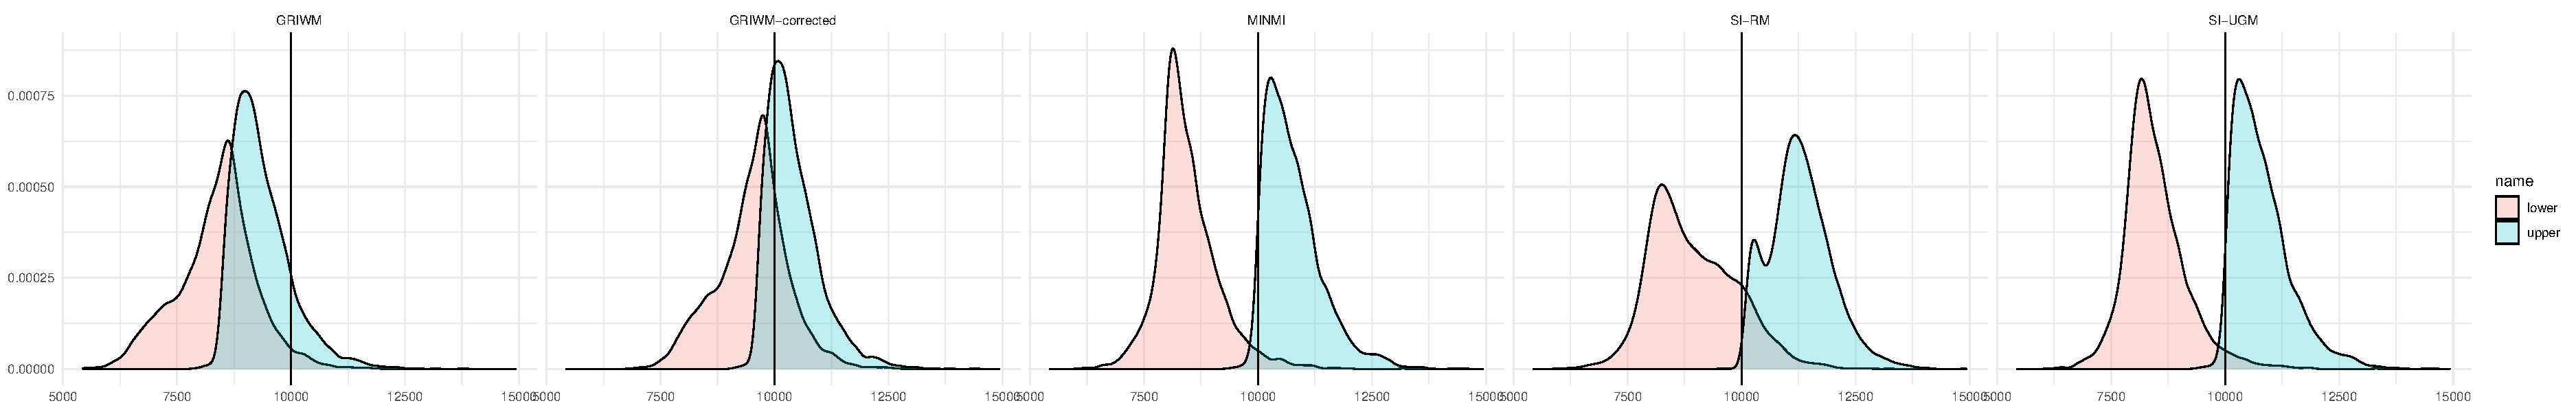
\includegraphics{sim_exp-results_files/figure-latex/unnamed-chunk-6-1.pdf}

\begin{Shaded}
\begin{Highlighting}[]
\ControlFlowTok{for}\NormalTok{ (i }\ControlFlowTok{in} \DecValTok{1}\SpecialCharTok{:}\FunctionTok{length}\NormalTok{(metrics)) \{}
  \FunctionTok{ggsave}\NormalTok{(}\AttributeTok{plot =}\NormalTok{ performance.point\_estimates.plots[[i]],}
         \AttributeTok{file =} \FunctionTok{paste0}\NormalTok{(}\StringTok{"../figures/plot{-}sim{-}exp{-}point{-}est{-}"}\NormalTok{, metrics[i], }\StringTok{".svg"}\NormalTok{),}
         \AttributeTok{dpi=}\DecValTok{320}\NormalTok{)}
\NormalTok{\}}
\end{Highlighting}
\end{Shaded}

\begin{verbatim}
## Saving 6.5 x 4.5 in image
## Saving 6.5 x 4.5 in image
## Saving 6.5 x 4.5 in image
## Saving 6.5 x 4.5 in image
\end{verbatim}

\begin{Shaded}
\begin{Highlighting}[]
\NormalTok{perf.point\_estimates.bias\_var.plot }\OtherTok{=}\NormalTok{ performance.point\_estimates.long }\SpecialCharTok{\%\textgreater{}\%}
  \FunctionTok{filter}\NormalTok{(Metric }\SpecialCharTok{\%in\%} \FunctionTok{c}\NormalTok{(}\StringTok{"Bias"}\NormalTok{, }\StringTok{"Variance"}\NormalTok{)) }\SpecialCharTok{\%\textgreater{}\%}
  \FunctionTok{ggplot}\NormalTok{(}\FunctionTok{aes}\NormalTok{(}\AttributeTok{x=}\NormalTok{Error, }\AttributeTok{y=}\NormalTok{value, }\AttributeTok{colour=}\FunctionTok{reorder}\NormalTok{(Method, value, }\AttributeTok{decreasing =}\NormalTok{ T))) }\SpecialCharTok{+}
  \FunctionTok{geom\_line}\NormalTok{() }\SpecialCharTok{+}
  \FunctionTok{geom\_point}\NormalTok{() }\SpecialCharTok{+}
  \FunctionTok{facet\_grid}\NormalTok{(Metric }\SpecialCharTok{\textasciitilde{}}\NormalTok{ Category, }\AttributeTok{scale=}\StringTok{"free\_y"}\NormalTok{) }\SpecialCharTok{+}
  \FunctionTok{labs}\NormalTok{(}\AttributeTok{colour =} \StringTok{"Method"}\NormalTok{, }\AttributeTok{y=}\ConstantTok{NULL}\NormalTok{) }\SpecialCharTok{+}
  \FunctionTok{theme\_bw}\NormalTok{()}

\NormalTok{perf.point\_estimates.bias\_var.plot}
\end{Highlighting}
\end{Shaded}

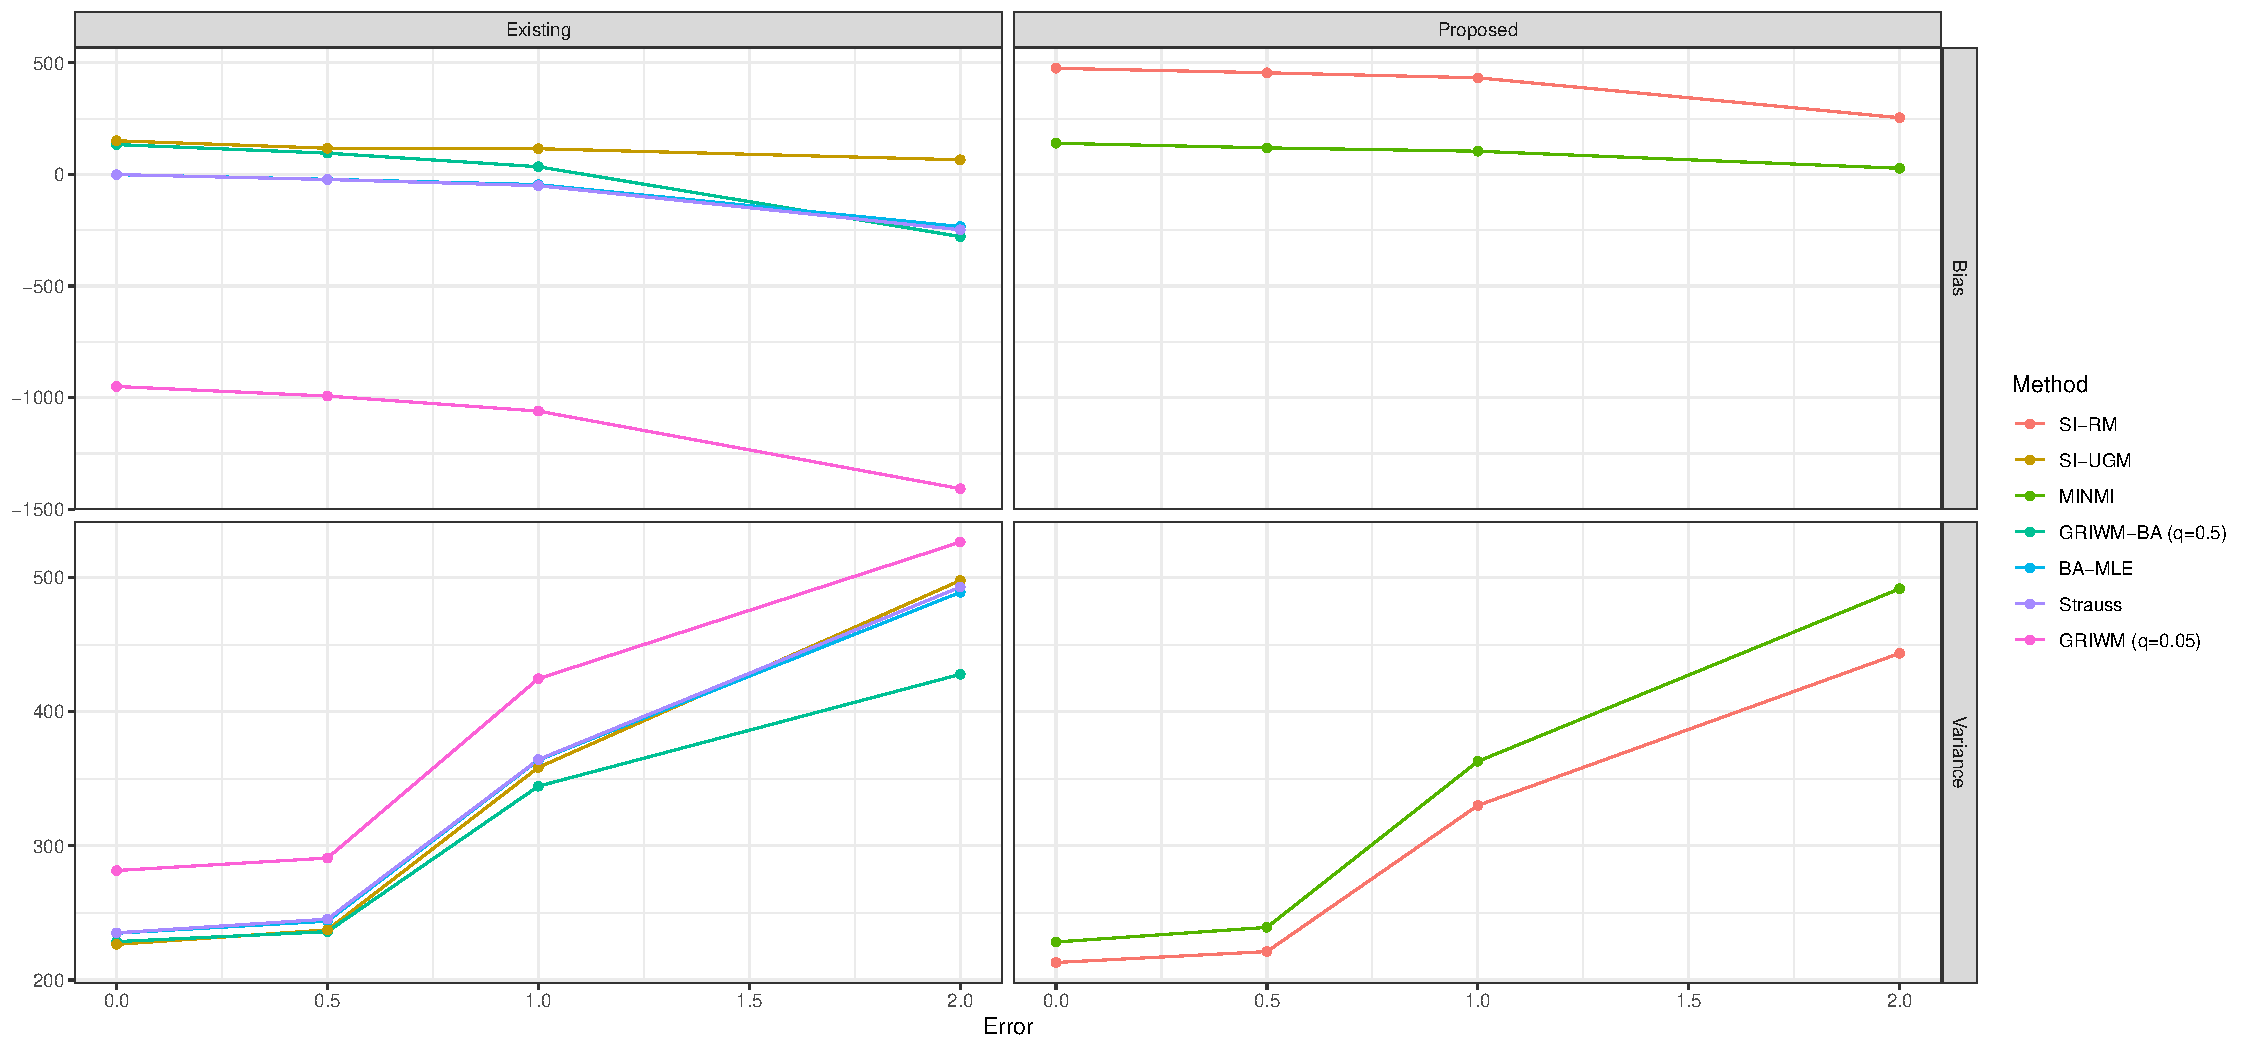
\includegraphics{sim_exp-results_files/figure-latex/unnamed-chunk-8-1.pdf}

\begin{Shaded}
\begin{Highlighting}[]
\FunctionTok{ggsave}\NormalTok{(}\AttributeTok{plot =}\NormalTok{ perf.point\_estimates.bias\_var.plot,}
       \AttributeTok{file =} \StringTok{"../figures/plot{-}sim{-}exp{-}point{-}est{-}Bias{-}Variance.svg"}\NormalTok{,}
       \AttributeTok{width=}\DecValTok{15}\NormalTok{, }\AttributeTok{height=}\DecValTok{7}\NormalTok{,}
       \AttributeTok{dpi =} \DecValTok{320}\NormalTok{)}
\end{Highlighting}
\end{Shaded}

\hypertarget{confidence-intervals}{%
\subsubsection{Confidence Intervals}\label{confidence-intervals}}

\begin{Shaded}
\begin{Highlighting}[]
\FunctionTok{options}\NormalTok{(}\AttributeTok{scipen =} \DecValTok{9}\NormalTok{)}
\ControlFlowTok{for}\NormalTok{ (metric }\ControlFlowTok{in} \FunctionTok{c}\NormalTok{(}\StringTok{"Coverage"}\NormalTok{, }\StringTok{"Average Width"}\NormalTok{, }\StringTok{"Average Runtime"}\NormalTok{)) \{}
\NormalTok{  experiment.results.conf\_int }\OtherTok{=}\NormalTok{ performance.conf\_int\_estimates }\SpecialCharTok{\%\textgreater{}\%}
    \FunctionTok{select}\NormalTok{(}\FunctionTok{c}\NormalTok{(method, error\_factor, }\FunctionTok{one\_of}\NormalTok{(metric))) }\SpecialCharTok{\%\textgreater{}\%}
    \FunctionTok{pivot\_wider}\NormalTok{(}
      \AttributeTok{id\_cols =}\NormalTok{ method,}
      \AttributeTok{names\_from =}\NormalTok{ error\_factor,}
      \AttributeTok{values\_from =} \FunctionTok{one\_of}\NormalTok{(metric),}
      \AttributeTok{names\_prefix =} \FunctionTok{paste}\NormalTok{(metric, }\StringTok{"| error = sigma*"}\NormalTok{)}
\NormalTok{    ) }\SpecialCharTok{\%\textgreater{}\%}
    \FunctionTok{arrange}\NormalTok{(}\SpecialCharTok{!!}\FunctionTok{syms}\NormalTok{(}\FunctionTok{paste}\NormalTok{(metric, }\StringTok{"| error = sigma*0"}\NormalTok{)))}
  \FunctionTok{print}\NormalTok{(}\FunctionTok{kable}\NormalTok{(experiment.results.conf\_int))}
  
\NormalTok{  experiment.results.kbl }\OtherTok{=}\NormalTok{ experiment.results.conf\_int }\SpecialCharTok{\%\textgreater{}\%}
    \FunctionTok{kable}\NormalTok{(}
      \AttributeTok{col.names =} \FunctionTok{c}\NormalTok{(}\StringTok{""}\NormalTok{, }\FunctionTok{paste0}\NormalTok{(}\FunctionTok{c}\NormalTok{(}\DecValTok{0}\NormalTok{, }\FloatTok{0.5}\NormalTok{, }\DecValTok{1}\NormalTok{, }\DecValTok{2}\NormalTok{), r}\StringTok{"\{*$\textbackslash{}sigma$\}"}\NormalTok{)),}
      \AttributeTok{booktabs =}\NormalTok{ T,}
      \AttributeTok{format =} \StringTok{"latex"}\NormalTok{,}
      \AttributeTok{escape =} \ConstantTok{FALSE}
\NormalTok{    ) }\SpecialCharTok{\%\textgreater{}\%}
    \FunctionTok{add\_header\_above}\NormalTok{(}\FunctionTok{unlist}\NormalTok{(}\FunctionTok{lst}\NormalTok{(}\StringTok{"Method"} \OtherTok{=} \DecValTok{1}\NormalTok{,}\SpecialCharTok{!!}\AttributeTok{metric :=} \DecValTok{4}\NormalTok{)), }\AttributeTok{line =}\NormalTok{ F)}
  \FunctionTok{writeLines}\NormalTok{(}
\NormalTok{    experiment.results.kbl,}
    \FunctionTok{paste0}\NormalTok{(}
      \StringTok{"../figures/table{-}sim{-}exp{-}conf{-}int{-}"}\NormalTok{,}
      \FunctionTok{str\_replace}\NormalTok{(}\FunctionTok{tolower}\NormalTok{(metric), }\StringTok{" "}\NormalTok{, }\StringTok{"{-}"}\NormalTok{),}
      \StringTok{".tex"}
\NormalTok{    )}
\NormalTok{  )}
\NormalTok{\}}
\end{Highlighting}
\end{Shaded}

\begin{tabular}{l|r|r|r|r}
\hline
method & Coverage | error = sigma*0 & Coverage | error = sigma*0.5 & Coverage | error = sigma*2 & Coverage | error = sigma*1\\
\hline
SI-RM & 97.4 & 96.3 & 95.1 & 93.8\\
\hline
SI-UGM & 97.3 & 96.2 & 94.9 & 93.7\\
\hline
MINMI & 94.5 & 95.2 & 95.0 & 93.0\\
\hline
GRIWM-BA (q=0.5) & 0.0 & 49.9 & 80.6 & 69.5\\
\hline
GRIWM (q=0.05) & 0.0 & 7.0 & 22.6 & 13.9\\
\hline
\end{tabular}

\begin{tabular}{l|r|r|r|r}
\hline
method & Average Width | error = sigma*0 & Average Width | error = sigma*0.5 & Average Width | error = sigma*2 & Average Width | error = sigma*1\\
\hline
SI-RM & 2005.35 & 2097.43 & 2960.26 & 2346.11\\
\hline
SI-UGM & 1961.14 & 2091.09 & 2964.30 & 2351.53\\
\hline
MINMI & 1917.16 & 2066.21 & 2945.03 & 2325.84\\
\hline
GRIWM-BA (q=0.5) & 0.00 & 548.08 & 1949.67 & 1047.99\\
\hline
GRIWM (q=0.05) & 0.00 & 608.33 & 2163.50 & 1162.65\\
\hline
\end{tabular}

\begin{tabular}{l|r|r|r|r}
\hline
method & Average Runtime | error = sigma*0 & Average Runtime | error = sigma*0.5 & Average Runtime | error = sigma*2 & Average Runtime | error = sigma*1\\
\hline
SI-RM & 0.0564 & 0.0607 & 0.0599 & 0.0599\\
\hline
SI-UGM & 4.7066 & 2.3306 & 1.6801 & 1.9374\\
\hline
MINMI & 0.0000 & 0.0013 & 0.0021 & 0.0014\\
\hline
GRIWM-BA (q=0.5) & 13.8988 & 13.8825 & 13.9422 & 13.9010\\
\hline
GRIWM (q=0.05) & 2.3355 & 2.3589 & 2.3641 & 18.1072\\
\hline
\end{tabular}

\begin{Shaded}
\begin{Highlighting}[]
\NormalTok{estimates }\SpecialCharTok{\%\textgreater{}\%}
  \FunctionTok{filter}\NormalTok{(}\SpecialCharTok{!}\FunctionTok{is.na}\NormalTok{(lower)) }\SpecialCharTok{\%\textgreater{}\%}
  \FunctionTok{select}\NormalTok{(method, lower, upper) }\SpecialCharTok{\%\textgreater{}\%}
  \FunctionTok{pivot\_longer}\NormalTok{(}\AttributeTok{cols=}\FunctionTok{c}\NormalTok{(lower, upper)) }\SpecialCharTok{\%\textgreater{}\%}
  \FunctionTok{filter}\NormalTok{(}\SpecialCharTok{!}\FunctionTok{is.na}\NormalTok{(value)) }\SpecialCharTok{\%\textgreater{}\%}
  \FunctionTok{ggplot}\NormalTok{(}\FunctionTok{aes}\NormalTok{(}\AttributeTok{x=}\NormalTok{value, }\AttributeTok{fill=}\NormalTok{name)) }\SpecialCharTok{+}
  \FunctionTok{geom\_density}\NormalTok{(}\AttributeTok{alpha=}\FloatTok{0.25}\NormalTok{) }\SpecialCharTok{+}
  \FunctionTok{geom\_vline}\NormalTok{(}\FunctionTok{aes}\NormalTok{(}\AttributeTok{xintercept=}\NormalTok{theta.true)) }\SpecialCharTok{+}
  \FunctionTok{facet\_wrap}\NormalTok{(method }\SpecialCharTok{\textasciitilde{}}\NormalTok{ ., }\AttributeTok{nrow=}\DecValTok{1}\NormalTok{) }\SpecialCharTok{+}
  \FunctionTok{theme\_minimal}\NormalTok{() }\SpecialCharTok{+}
  \FunctionTok{labs}\NormalTok{(}\AttributeTok{x=}\ConstantTok{NULL}\NormalTok{, }\AttributeTok{y=}\ConstantTok{NULL}\NormalTok{)}
\end{Highlighting}
\end{Shaded}

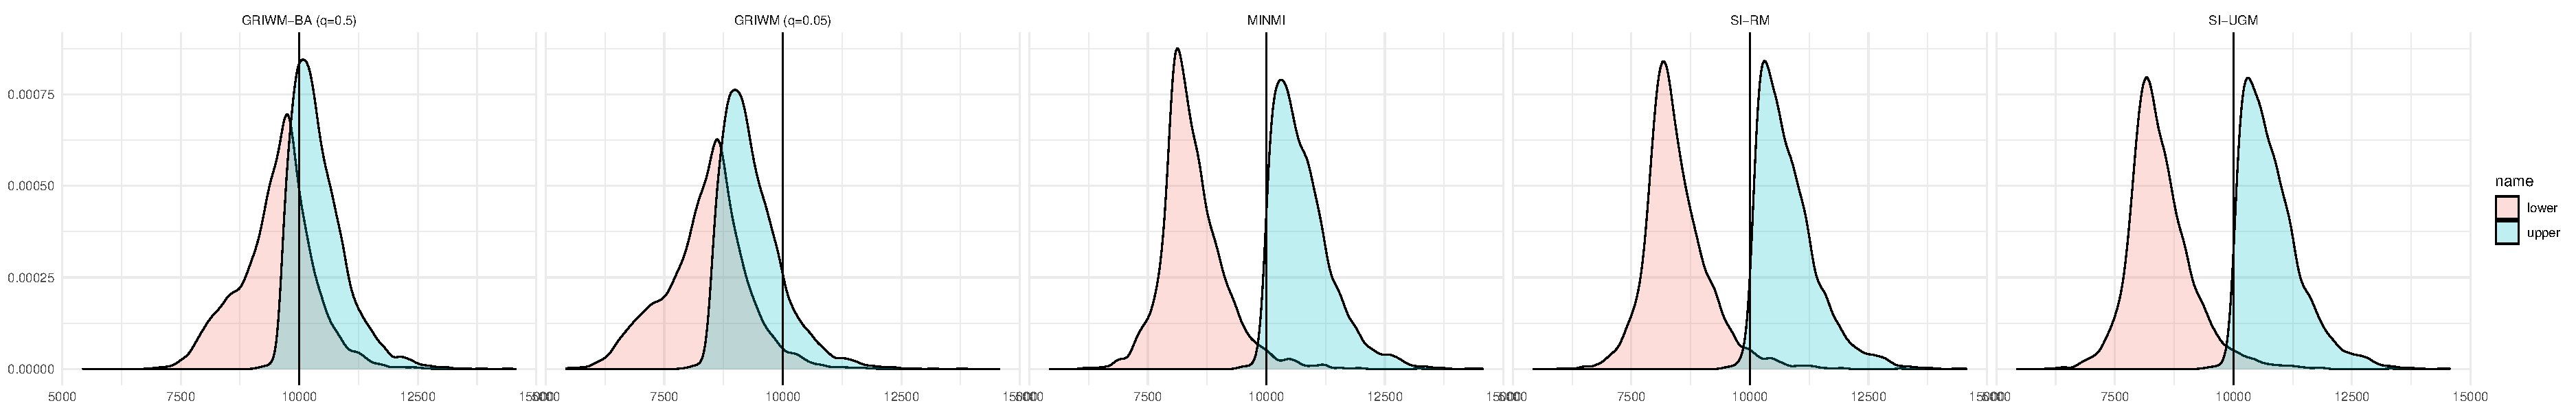
\includegraphics{sim_exp-results_files/figure-latex/unnamed-chunk-11-1.pdf}

\begin{Shaded}
\begin{Highlighting}[]
\NormalTok{p }\OtherTok{=}\NormalTok{ estimates }\SpecialCharTok{\%\textgreater{}\%}
  \FunctionTok{filter}\NormalTok{(}\SpecialCharTok{!}\FunctionTok{is.na}\NormalTok{(lower) }\SpecialCharTok{\&}\NormalTok{ error\_factor }\SpecialCharTok{==} \DecValTok{1}\NormalTok{) }\SpecialCharTok{\%\textgreater{}\%}
  \FunctionTok{group\_by}\NormalTok{(method\_cat, method) }\SpecialCharTok{\%\textgreater{}\%}
  \FunctionTok{summarise}\NormalTok{(}\AttributeTok{lower =} \FunctionTok{mean}\NormalTok{(lower), }\AttributeTok{upper=}\FunctionTok{mean}\NormalTok{(upper), }\AttributeTok{point=}\FunctionTok{mean}\NormalTok{(point)) }\SpecialCharTok{\%\textgreater{}\%}
  \FunctionTok{mutate}\NormalTok{(}\AttributeTok{width=}\NormalTok{upper}\SpecialCharTok{{-}}\NormalTok{lower) }\SpecialCharTok{\%\textgreater{}\%}
  \FunctionTok{mutate}\NormalTok{(}\AttributeTok{method\_cat\_int =} \FunctionTok{ifelse}\NormalTok{(method\_cat }\SpecialCharTok{==} \StringTok{"Existing"}\NormalTok{, }\DecValTok{0}\NormalTok{, }\DecValTok{1}\NormalTok{)) }\SpecialCharTok{\%\textgreater{}\%}
  \FunctionTok{ggplot}\NormalTok{(}\FunctionTok{aes}\NormalTok{(}\AttributeTok{colour=}\NormalTok{method\_cat)) }\SpecialCharTok{+}
  \FunctionTok{geom\_pointrange}\NormalTok{(}\FunctionTok{aes}\NormalTok{(}\AttributeTok{xmin=}\NormalTok{lower, }\AttributeTok{xmax=}\NormalTok{upper, }\AttributeTok{x=}\NormalTok{point, }\AttributeTok{y=}\FunctionTok{reorder}\NormalTok{(method, method\_cat\_int))) }\SpecialCharTok{+}
  \FunctionTok{guides}\NormalTok{(}\AttributeTok{colour =} \FunctionTok{guide\_legend}\NormalTok{(}\AttributeTok{reverse=}\ConstantTok{TRUE}\NormalTok{)) }\SpecialCharTok{+}
  \FunctionTok{labs}\NormalTok{(}\AttributeTok{y=}\ConstantTok{NULL}\NormalTok{, }\AttributeTok{x=}\StringTok{"Years (BP)"}\NormalTok{,}
       \AttributeTok{title=}\StringTok{"Simulation Experiment Confidence Intervals"}\NormalTok{,}
       \AttributeTok{colour=}\StringTok{"Method"}\NormalTok{,}
       \AttributeTok{subtitle=}\StringTok{"(Average of Interval Endpoints and Point Estimates)"}\NormalTok{) }\SpecialCharTok{+}
  \FunctionTok{scale\_x\_continuous}\NormalTok{(}\AttributeTok{breaks =} \FunctionTok{seq}\NormalTok{(}\AttributeTok{from=}\DecValTok{8000}\NormalTok{, }\AttributeTok{to=}\DecValTok{11500}\NormalTok{, }\AttributeTok{by=}\DecValTok{500}\NormalTok{)) }\SpecialCharTok{+}
  \FunctionTok{theme\_bw}\NormalTok{()}
\end{Highlighting}
\end{Shaded}

\begin{verbatim}
## `summarise()` has grouped output by 'method_cat'. You can override using the
## `.groups` argument.
\end{verbatim}

\begin{Shaded}
\begin{Highlighting}[]
\NormalTok{p}
\end{Highlighting}
\end{Shaded}

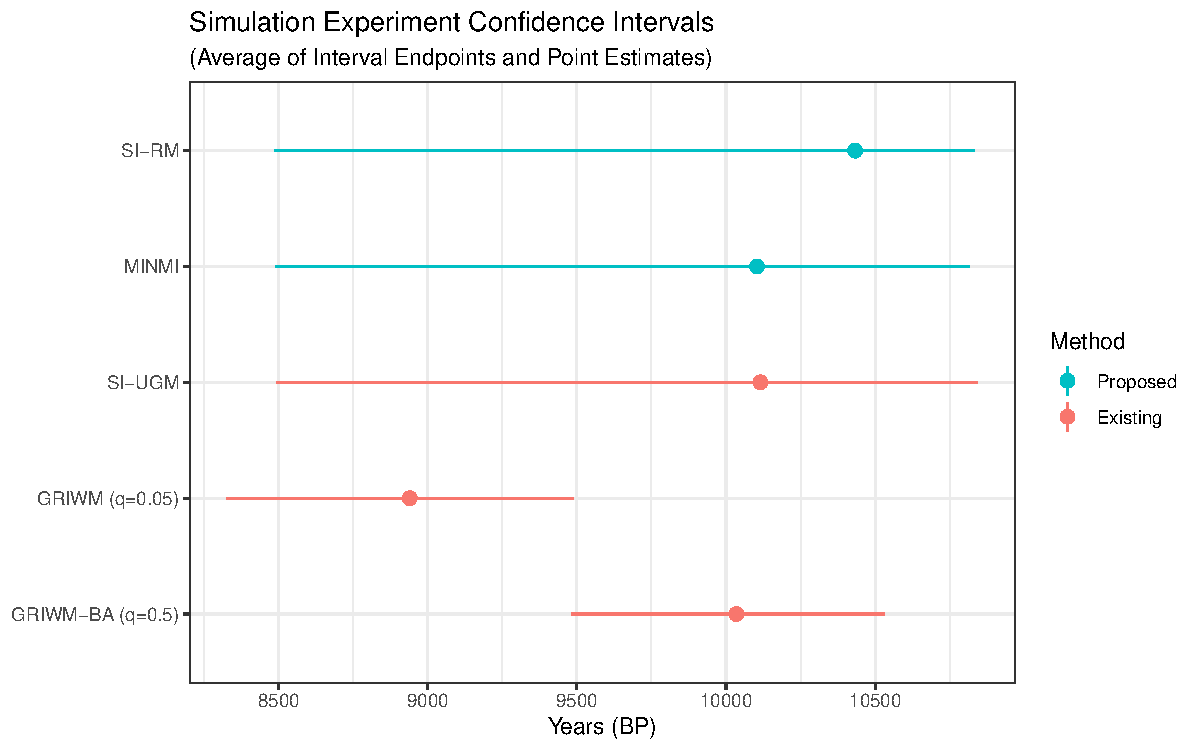
\includegraphics{sim_exp-results_files/figure-latex/unnamed-chunk-12-1.pdf}

\begin{Shaded}
\begin{Highlighting}[]
\FunctionTok{ggsave}\NormalTok{(}\AttributeTok{filename=}\StringTok{"../figures/sim{-}exp{-}intervals.svg"}\NormalTok{, }\AttributeTok{plot=}\NormalTok{p, }\AttributeTok{height=}\DecValTok{5}\NormalTok{, }\AttributeTok{width=}\DecValTok{8}\NormalTok{)}
\end{Highlighting}
\end{Shaded}

\hypertarget{monte-carlo-samples-for-minmi}{%
\subsection{Monte Carlo Samples for
MINMI}\label{monte-carlo-samples-for-minmi}}

\begin{Shaded}
\begin{Highlighting}[]
\NormalTok{B.minmi }\OtherTok{=} \FunctionTok{readRDS}\NormalTok{(}\StringTok{"../data/sim\_exp{-}B{-}minmi.RDS"}\NormalTok{)}
\NormalTok{B.minmi }\OtherTok{=}\NormalTok{ B.minmi }\SpecialCharTok{\%\textgreater{}\%} \FunctionTok{arrange}\NormalTok{(error\_factor) }\SpecialCharTok{\%\textgreater{}\%} \FunctionTok{mutate}\NormalTok{(}\AttributeTok{error\_factor =} \FunctionTok{paste0}\NormalTok{(error\_factor, r}\StringTok{"\{*$\textbackslash{}sigma$\}"}\NormalTok{))}

\NormalTok{B.minmi.kbl }\OtherTok{=}\NormalTok{ B.minmi }\SpecialCharTok{\%\textgreater{}\%}
  \FunctionTok{filter}\NormalTok{(error\_factor }\SpecialCharTok{!=} \DecValTok{0}\NormalTok{) }\SpecialCharTok{\%\textgreater{}\%}
  \FunctionTok{kable}\NormalTok{(}\AttributeTok{col.names =} \FunctionTok{c}\NormalTok{(}\StringTok{"Variation"}\NormalTok{, }\StringTok{"$q = 0.025$"}\NormalTok{, }\StringTok{"$q = 0.5$"}\NormalTok{, }\StringTok{"$q = 0.975$"}\NormalTok{),}
        \AttributeTok{booktabs=}\NormalTok{T, }\AttributeTok{format=}\StringTok{"latex"}\NormalTok{, }\AttributeTok{escape =} \ConstantTok{FALSE}\NormalTok{) }\SpecialCharTok{\%\textgreater{}\%}
  \FunctionTok{add\_header\_above}\NormalTok{(}\FunctionTok{c}\NormalTok{(}\StringTok{\textasciigrave{}}\AttributeTok{Measurement Error}\StringTok{\textasciigrave{}}\OtherTok{=}\DecValTok{1}\NormalTok{, }\StringTok{\textasciigrave{}}\AttributeTok{$B$}\StringTok{\textasciigrave{}}\OtherTok{=}\DecValTok{3}\NormalTok{), }\AttributeTok{line=}\NormalTok{F)}

\FunctionTok{print}\NormalTok{(B.minmi.kbl)}
\end{Highlighting}
\end{Shaded}

\begin{verbatim}
## 
## \begin{tabular}{lrrr}
## \toprule
## \multicolumn{1}{c}{Measurement Error} & \multicolumn{3}{c}{\$B\$} \\
## Variation & $q = 0.025$ & $q = 0.5$ & $q = 0.975$\\
## \midrule
## 0*$\sigma$ & 2 & 2 & 2\\
## 0.5*$\sigma$ & 5 & 6 & 3\\
## 1*$\sigma$ & 14 & 24 & 9\\
## 2*$\sigma$ & 42 & 91 & 33\\
## 4*$\sigma$ & 136 & 243 & 119\\
## \bottomrule
## \end{tabular}
\end{verbatim}

\begin{Shaded}
\begin{Highlighting}[]
\FunctionTok{writeLines}\NormalTok{(B.minmi.kbl, }\StringTok{"../figures/table{-}sim{-}exp{-}minmi{-}Bs.tex"}\NormalTok{)}
\end{Highlighting}
\end{Shaded}


\end{document}
